\documentclass[../Main.tex]{subfiles}

\begin{document}
\author{Electromagnetic Waves} %use author for title of lesson
\date{Year 1 Topics 16,17} %use date to refer to topic in main booklet

\section{EM Waves} %Section is the title of the lesson repeated, ready for the main contents page.

\begin{frame}{Electromagnetic Spectrum}
    \begin{figure}
        \centering
        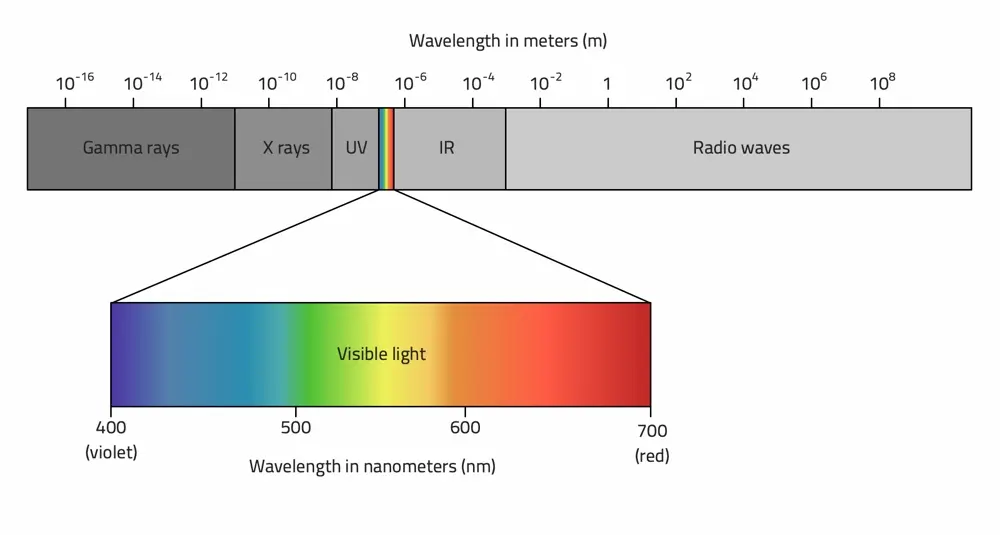
\includegraphics[width=0.9\textwidth]{Waves_Images/EMspectrum.png}
    \end{figure}
    You need to know the parts of the EM-spectrum, how they relate in terms of wavelength/frequency, and the approx wavelengths for visible light.
\end{frame}

\begin{frame}{Electromagnetic Spectrum}
    All parts of the EM spectrum are electromagnetic waves. They do not require a medium to travel through and ALL have the same wave speed - equal to the speed of light, which is given to you in your formula book.
    
    \begin{equation*}
        c=3.00 \times 10^ 8 ms^{-1}
    \end{equation*} (or to be exact c=299,792,458ms$^{-1}$)\footnote{I will be testing you!} \newline
    
    EM waves are transverse, formed of alternate electric and magnetic fields perpendicular to each other (more on this in module 6)
    \begin{figure}
        \centering
        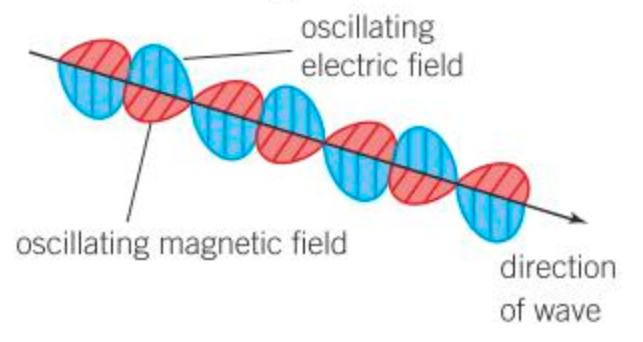
\includegraphics[height=2.5cm]{Waves_Images/emwavefields.png}
    \end{figure}
\end{frame}

\begin{frame}{Studying the Universe}
    EM waves are how we can study the Universe. We can set up cameras/sensors for all types of EM wave. Problem is, not all types of EM wave can be detected from the surface of Earth, and for those that do there are plenty of problems involved with them.
    
    \begin{figure}
        \centering
        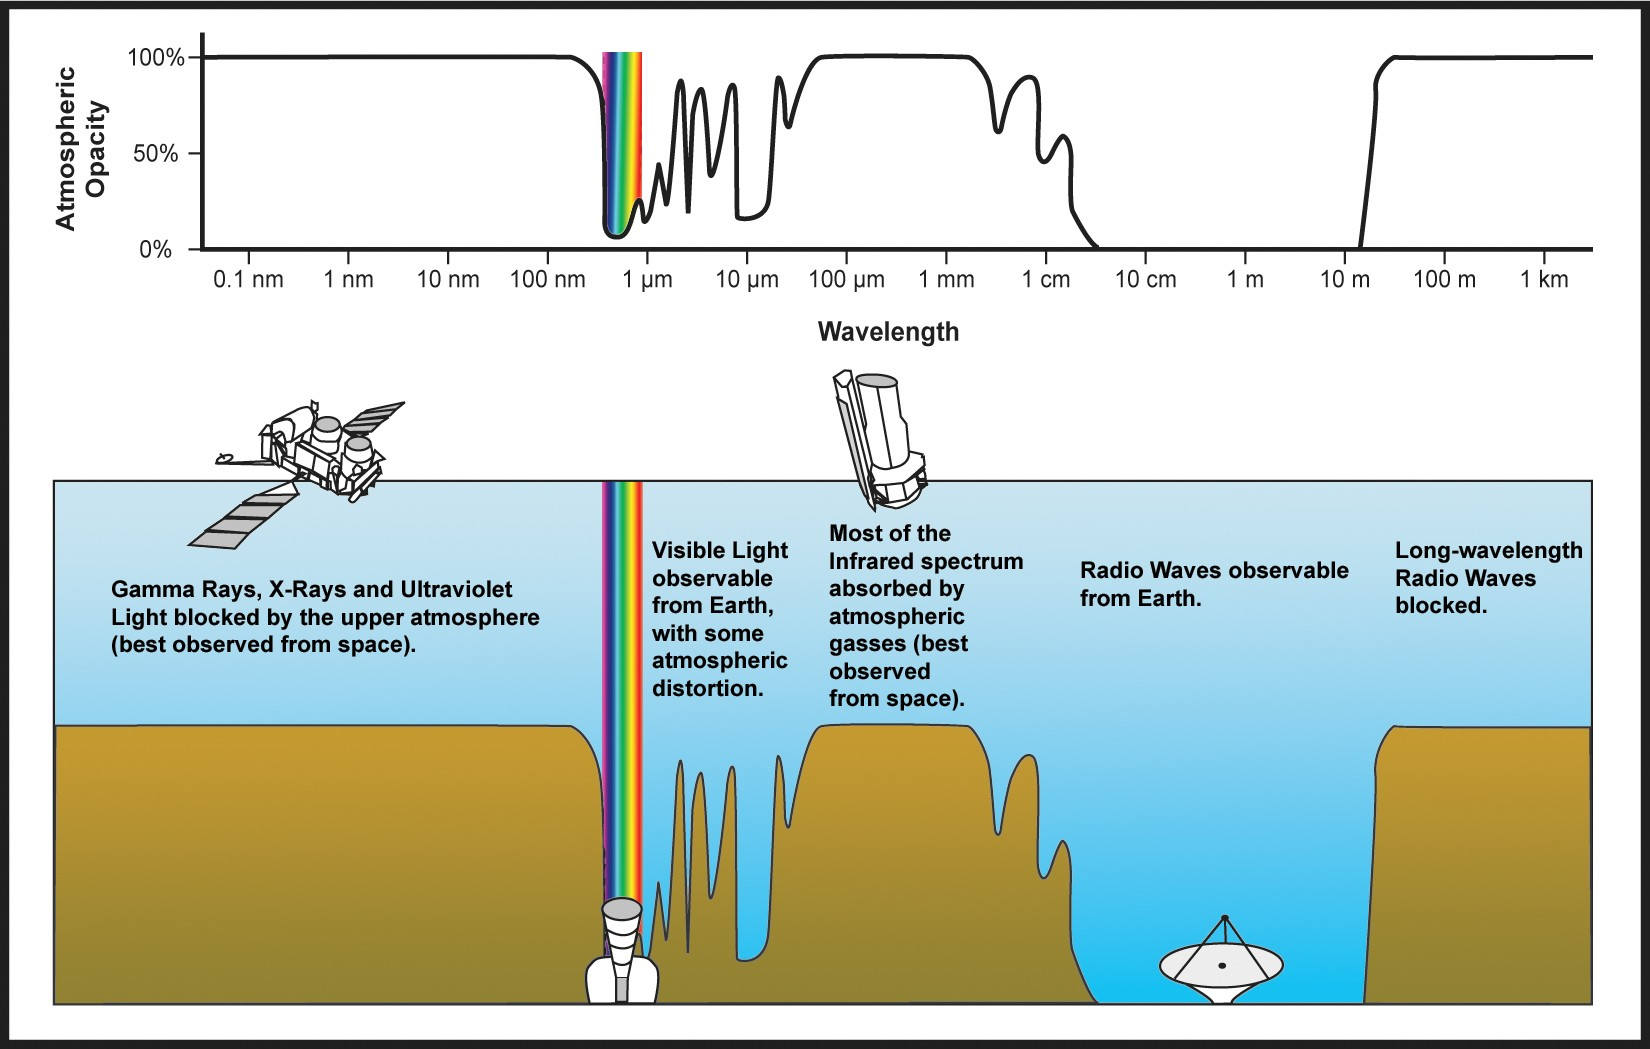
\includegraphics[height=5cm]{Waves_Images/atmosphereopacity.png}
    \end{figure}
\end{frame}

\begin{frame}{Polarisation}
    Light emitted from a source can have oscillations that are at any angle (though still remaining perpendicular to the direction of travel). This remains true for all transverse waves, not just light which is most common.
    
    \begin{figure}
        \centering
        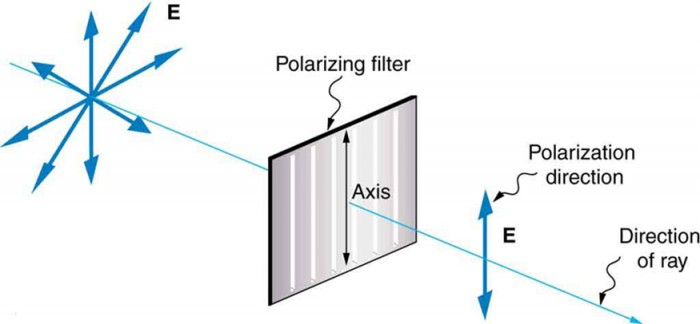
\includegraphics[width=6cm]{Waves_Images/1polarisingfilter.png}
    \end{figure}
    
    Through a polarising filter, this light can be polarised, by which is meant that all the waves transmitted have oscillation in a single plane - all others are blocked.
\end{frame}

\begin{frame}{Polarisation}
    If polarised light is passed through another polarising filter that is help perpendicular to the original filter, what do we think might happen? \pause
    
    \begin{figure}
        \centering
        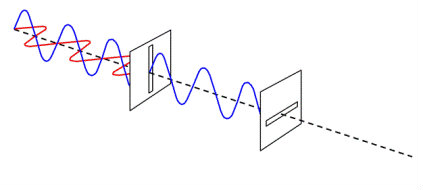
\includegraphics[height=4cm]{Waves_Images/2polarisingfilter.png}
    \end{figure}
    
    The polarised light can no longer pass through the second polarised filter as that plane is blocked by the filter.
\end{frame}

\begin{frame}{Polarisation}
    Light that is be reflected off a road surface, or a body of water, may be partially polarised. When observed through a polarising filter, this light becomes fully polarised, perhaps even removed entirely.
    
    \begin{figure}
        \centering
        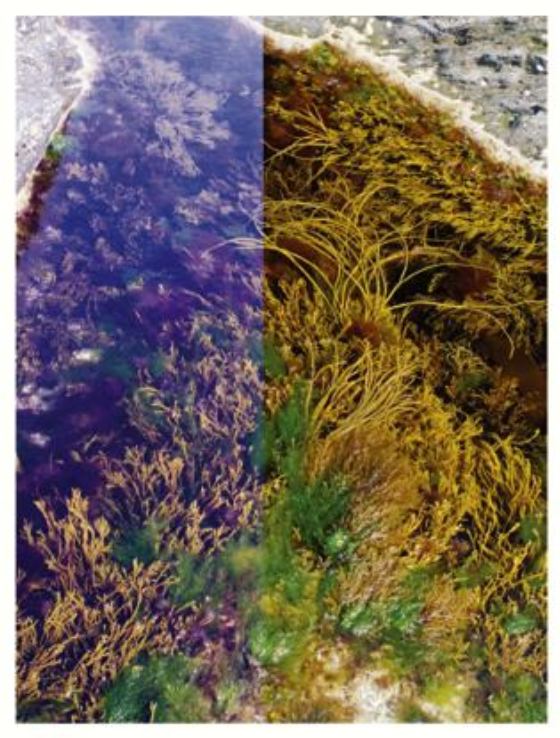
\includegraphics[height=4cm]{Waves_Images/polarisingglasses.png}
    \end{figure}
\end{frame}

\begin{frame}{Intensity of a wave}
    The intensity of a wave is given by the radiant power delivered across a surface area. This is most commonly found in terms of light intensity, but is true for all waves.
    
    \begin{equation*}
        I = \frac{P}{A}
    \end{equation*}
    
    What might the units for this be? \pause
    -- $Wm^{-2}$. \newline
    
    Since we generally take light to originate from a point source, it will always spread out equally in all directions. You can imagine a sphere of radius r around the source. The surface area of the sphere is given by 
    
    \begin{equation*}
        A = 4\pi r^2
    \end{equation*}
    
    Hence the intensity is \begin{equation*}
        I = \frac{P}{4\pi r^2}
    \end{equation*}
\end{frame}

\begin{frame}{Example}
\begin{figure}
    \centering
    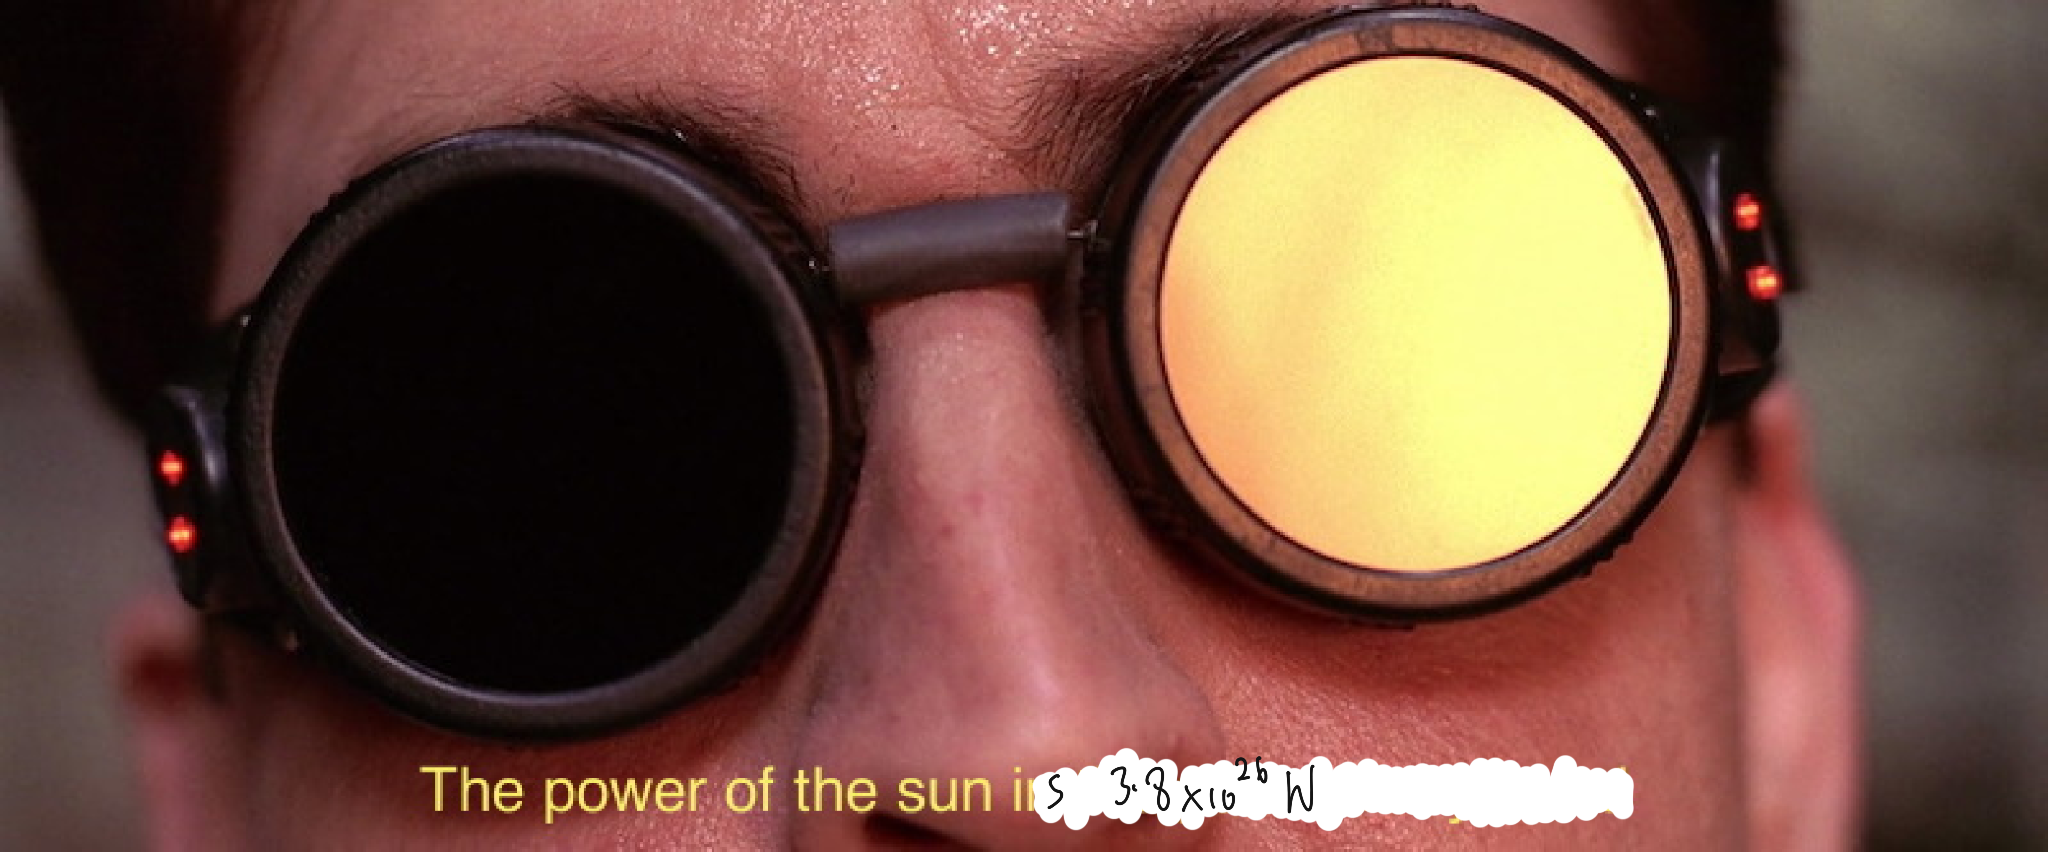
\includegraphics[width=\textwidth]{Waves_Images/powerofthesun.png}
\end{figure}
    \begin{exampleblock}{Example}
    The power of the Sun is $3.8\times 10^{26}$ W, and the average distance between the Earth and Sun is 150 million km. Calculate the intensity of the radiation falling on Earth. \pause
    -- $1300 Wm^{-2}$.
    \end{exampleblock}
\end{frame}

\begin{frame}{Inverse-square law}
    Given that a light source tends to be constant in power, the only remaining variable for light intensity is the distance from the source, r.
    
    \begin{equation*}
        I \propto \frac{1}{r^2}
    \end{equation*} -- this is known as the inverse-square law. Or in other words, increasing the radius by 2, reduces the received light intensity by a factor of 4.
    \pause
    \begin{exampleblock}{Example}
    On Mars, a distance of 230 million km from the Sun, the intensity of radiation falling on the surface is 570 $Wm^{-2}$. Jupiter is 780 million km away from the Sun. Determine the intensity of light received at Jupiter. \pause
    --$50Wm^{-2}$.
    \end{exampleblock} \pause
    
    \begin{exampleblock}{Example 2}
    The New Horizons probe is currently 8 billion km away from the Sun. Determine the intensity of radiation that would be received by the New Horizons probe \pause 
    0.47 $Wm^{-2}$.
    \end{exampleblock}
\end{frame}

\begin{frame}{Inverse-square law}
    Given that a light source tends to be constant in power, the only remaining variable for light intensity is the distance from the source, r.
    
    \begin{equation*}
        I \propto \frac{1}{r^2}
    \end{equation*} -- this is known as the inverse-square law. Or in other words, increasing the radius by 2, reduces the received light intensity by a factor of 4.
    
    
    \begin{exampleblock}{Example 2}
    The New Horizons probe is currently 8 billion km away from the Sun. Determine the intensity of radiation that would be received by the New Horizons probe 
    0.47 $Wm^{-2}$.
    \end{exampleblock}
    
    \begin{exampleblock}{Example 2b}
    The New Horizons probe requires 250W of power. Calculate the area of the solar panel that would be required to power the probe at this distance. \pause 
    --$530m^2$. (This is $\sim$equivalent to floor area of the SHUB x3!)
    \end{exampleblock}
\end{frame}

\end{document}